\documentclass{article}
\usepackage[letterpaper]{geometry}
\usepackage{graphicx}
\usepackage{xcolor}
\usepackage{amsmath}

% typesetting
% Margins and typesetting
\setlength{\textwidth}{5.00in}
\setlength{\oddsidemargin}{3.25in}
\addtolength{\oddsidemargin}{-0.5\textwidth}
\addtolength{\topmargin}{-0.55in}
\addtolength{\textheight}{2.00in}
\linespread{1.08}
\pagestyle{myheadings}
\markboth{}{\color{gray}\sffamily Hogg \& Villar / \texttt{MNIST-plus-plus}}
\sloppy\sloppypar\raggedbottom\frenchspacing
\renewcommand{\paragraph}[1]{\par\medskip\noindent\textbf{#1} ---}

\title{\bfseries \texttt{MNIST++}: Benchmarks for equivariant learning and reasoning tasks}
\author{David W. Hogg \& Soledad Villar}
\date{}

\begin{document}

\maketitle

\begin{abstract}\noindent
    The objective of this paper is to introduce data, code and benchmarks for simple equivariant classification, regression, and reasoning tasks.
    We provide four datasets and seven learning tasks based on simple tranformations of the MNIST and Fashion-MNIST datasets.
    Some of the learning tasks are to recognize objects and handwritten digits in images that have had geometric transformations applied; some are to identify the geometric transformations themselves.
    The images are designed to contain enough context to determine (in most cases) both the image contents and the geometric transformations.
    We train standard-issue CNNs to deliver baseline performances on the learning tasks.
    One of the tasks---\texttt{MNIST+4}---involves identifying ordered sets of numbers in a transformed image; it is a true reasoning task and is therefore expected to be challenging for contemporary machine-learning methods.
\end{abstract}

\section{Introduction}

Real-world learning tasks may require to identify objects in arbitrary orientations and make inference depending on contexts. 
See Figure~\ref{fig:example} for an example image and recognition task in this category.
The objective of this work is to provide toy datasets for these tasks. 

Describe, cite and honor MNIST. Also Fashion-MNIST.

BUT: In natural images text can appear with different shears and orientations.
Therefore it is natural to considered a transformed version of MNIST. However, handwritten digits may not be identifiable after rotations or reflections (6s and 9s, 2s and 5s, or even 2s and 6s may look indistinguishable after these transformations).
In natural contexts, however, 6s and 9s are not read in isolation; they are read as part of a document or signage context where orientation can be inferred from surrounding characters and features.
Thus we can make a dataset that is invariant to rotations, but which includes enough contextual information to determine orientations and parities.

We have made four datasets and seven learning tasks, all of which are designed to be swap-in replacements for MNIST and Fashion-MNIST.
We have trained some standard CNNs to provide baseline performance on all seven tasks.
These baselines should be easy to crush.

\section{Datasets and learning tasks}

\subsection*{Dataset 1: \texttt{Fashion++}}
The Fashion-MNIST-plus dataset takes the Fashion-MNIST data and subject it to random rotations and reflections. This is a natural classification task since clothing doesn't have a preferred orientation.

\begin{figure}[t!]
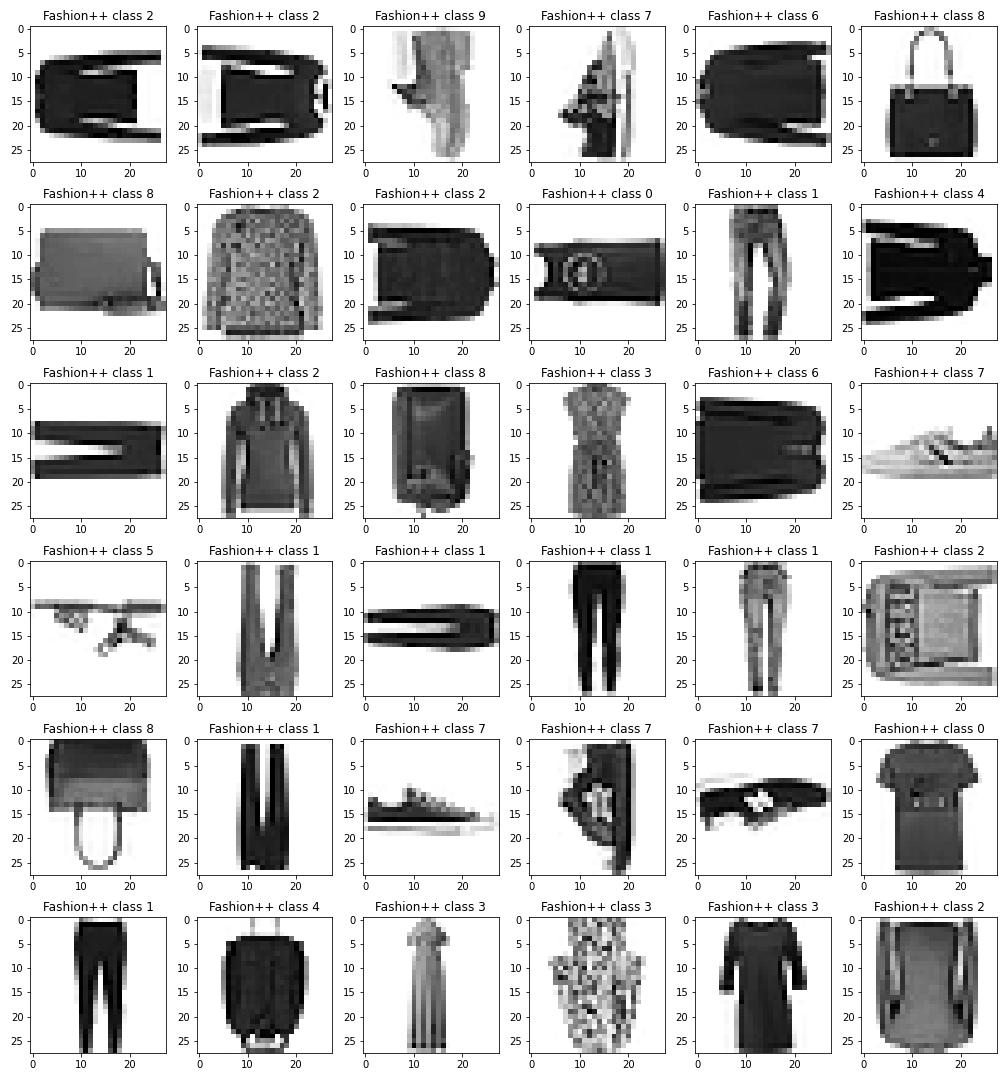
\includegraphics[width=\textwidth]{../notebooks/Fashion++.png}
\caption{The first 36 training-set images from the \texttt{Fashion++} dataset.\label{fig:f}}
\end{figure}

\paragraph{Learning task 1: \texttt{Fashion++} labels}
Identify the labels (classification).

\subsection*{Dataset 2: \texttt{MNIST+4}}

\begin{figure}[t!]
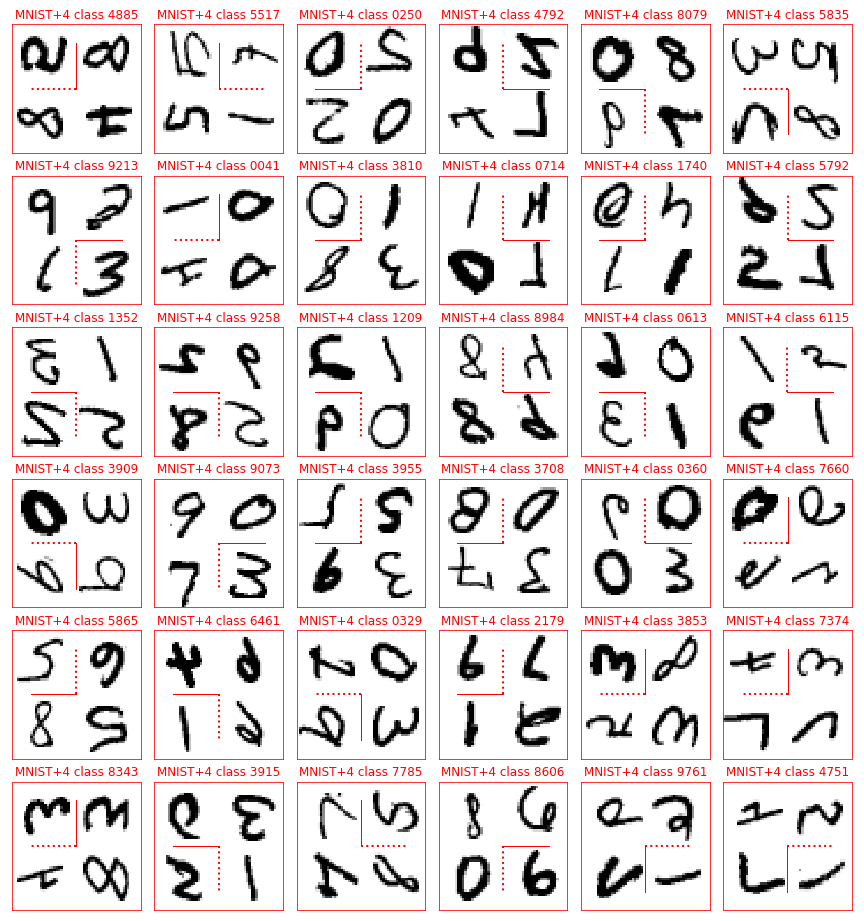
\includegraphics[width=\textwidth]{../notebooks/MNIST+4.png}
\caption{foo and bar.\label{fig:4}}
\end{figure}

\paragraph{Learning task 2: \texttt{MNIST+4} labels}
Identify the labels (classification and reasoning).
This has a reasoning component; note that some labels in the test set don't exist in the training set.
And yet humans can crush this (ish).

\paragraph{Learning task 3: \texttt{MNIST+4} group elements}
Foo and bar.

\subsection*{Dataset 3: \texttt{MNIST+9}}

\begin{figure}[t!]
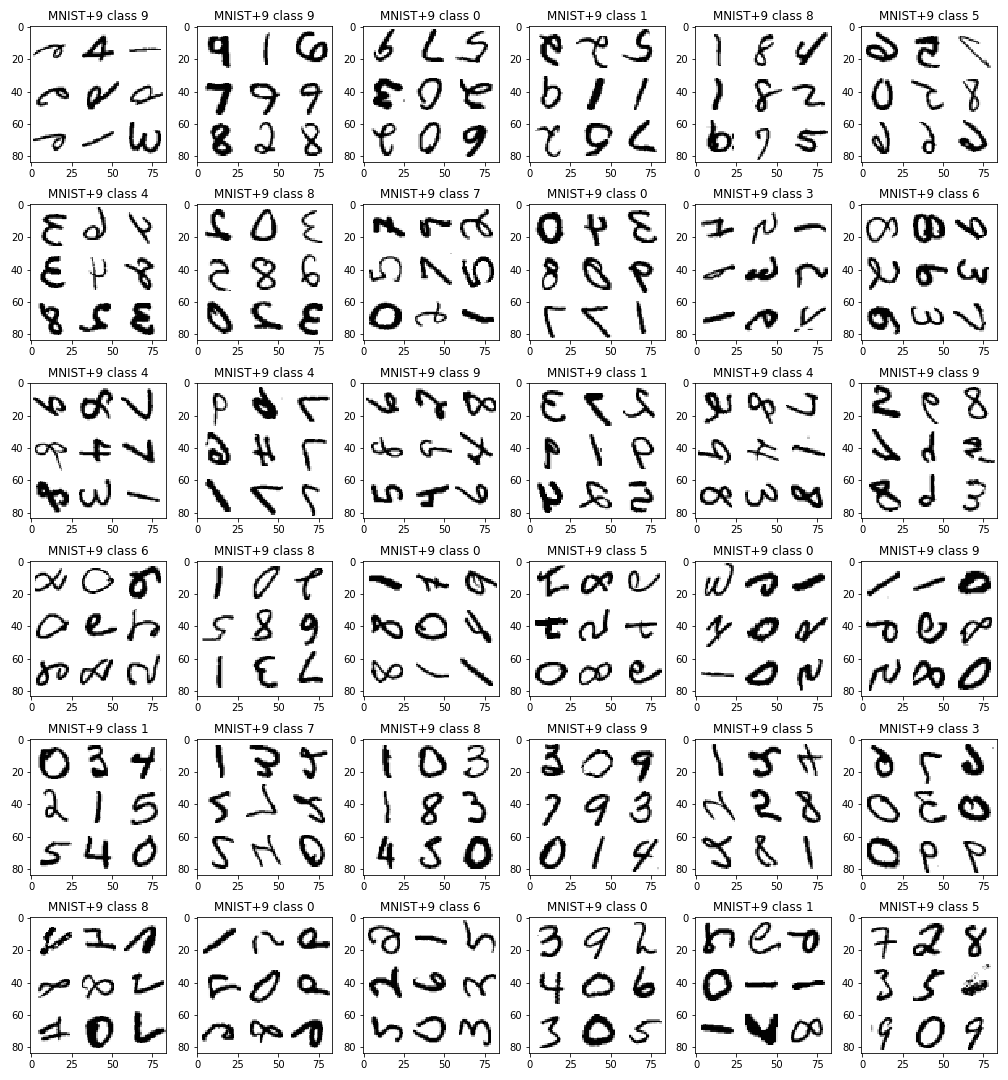
\includegraphics[width=\textwidth]{../notebooks/MNIST+9.png}
\caption{foo and bar.\label{fig:9}}
\end{figure}

\paragraph{Learning task 4: \texttt{MNIST+9} central digit labels}
Identify the labels (classification and reasoning).

\paragraph{Learning task 5: \texttt{MNIST+9} group elements}
Foo and bar.

\subsection*{Dataset 4: \texttt{MNIST+Inf}}

\begin{figure}[t!]
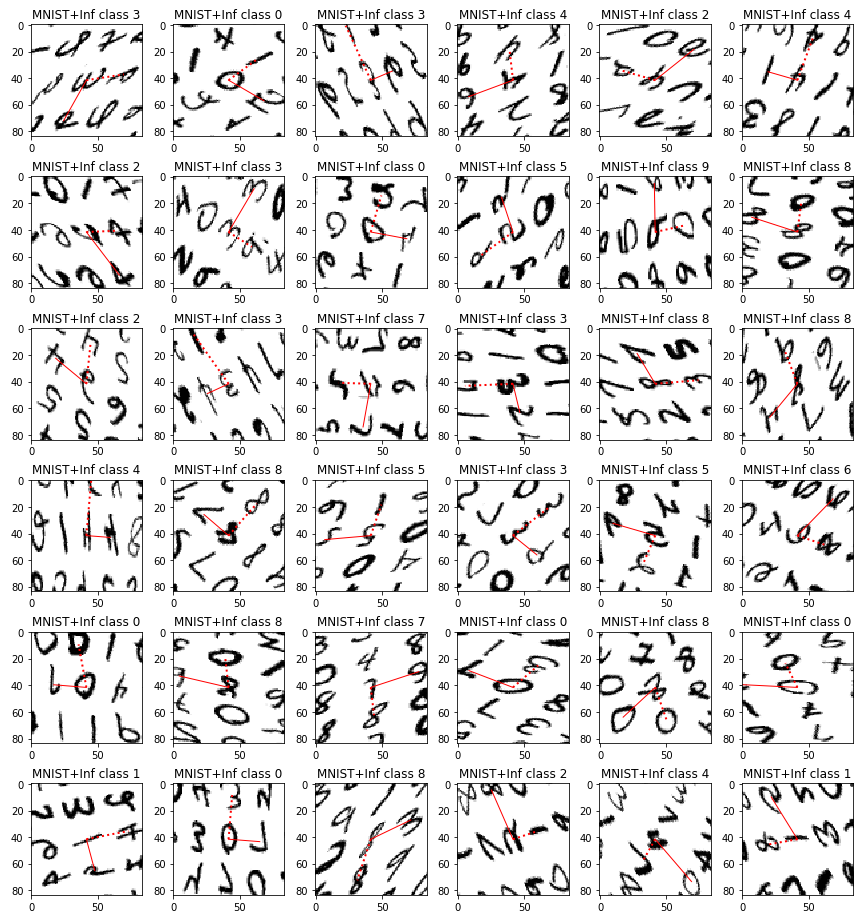
\includegraphics[width=\textwidth]{../notebooks/MNIST+Inf.png}
\caption{foo and bar.\label{fig:Inf}}
\end{figure}

\paragraph{Learning task 4: \texttt{MNIST+Inf} central digit labels}
Identify the labels (classification and reasoning).

\paragraph{Learning task 5: \texttt{MNIST+Inf} linear transformation operators}
Foo and bar. This is a regression!

\section{Baselines}

\section{Data download and discussion}

How do I get the data?

Comments about data augmentation.

Comments about reasoning?

\paragraph{Acknowledgements}
It is a pleasure to thank
  Wilson Gregory (JHU)
for valuable discussions.
SOLE GRANT NUMBERS.

\bibliographystyle{plain}
\raggedright
\bibliography{dipole}

\end{document}
